\chapter{Preliminares}\label{Chapter2}

\section{Computación cuántica}

La computación cuántica es un paradigma de computación que utiliza fenómenos de la mecánica cuántica, como la superposición y el entrelazamiento, lo que da lugar a puertas lógicas no presentes en la computación clásica. Esto permite que se puedan crear nuevos algoritmos, algunos de los cuales poseen ganancias de complejidad considerables frente a sus equivalente clásicos. Un ejemplo interesante es el algoritmo de Shor, el cual permite factorizar enteros en tiempo polinomial, mientras que el mejor algoritmo clásico conocido lo hace en tiempo sub-exponencial.

En la computación cuántica, la información se representa con vectores normalizados en espacios de Hilbert. Para nuestro trabajo, es suficiente considerar los espacios definidos sobre números complejos, con una norma y un concepto de ortogonalidad.

El espacio más chico es el definido sobre \( \mathbb{C}^2 \). La base estándar de este espacio se denota como \( \{\ket{0}, \ket{1}\} \). Llamamos \textit{qubit} a un vector de la forma \( \alpha \ket{0} + \beta \ket{1} \) donde \( |\alpha|^2 + |\beta|^2 = 1 \). Por otra parte, como los qubits son vectores, se pueden representar utilizando cualquier otra base.

Un qubit de la forma \( \alpha \ket{0} + \beta \ket{1} \) se dice que está en una superposición de \( \ket{0} \) y \( \ket{1} \). A diferencia de la computación clásica, en la cual leer un bit no conlleva ningún tipo de particularidad, en computación cuántica, leer un qubit se realiza utilizando una operación denominada \textit{medición} mediante la cual la superposición desaparece y el qubit colapsa a un estado particular, ya sea \( \ket{0} \) o \( \ket{1} \), o a algún otro si la operación de medición lo hace cambiar de base.
Si tenemos un qubit de la forma \( \alpha \ket{0} + \beta \ket{1} \), el medirlo en la base estándar hará que colapse al estado \( \ket{0} \) con probabilidad \( |\alpha|^2 \) o a \( \ket{1} \) con probabilidad \( |\beta|^2 \).

También podemos combinar espacios utilizando el denominado \textit{producto tensorial}, notado \( \tensor \). Esto permite representar sistemas de más de un qubit a la vez.
Por ejemplo, el espacio \( \mathbb{C}^2 \tensor \mathbb{C}^2 \) tiene base \( \{\ket{00}, \ket{01}, \ket{10} \ket{11}\} \) y un vector de dicha base tiene la forma \( \alpha \ket{00} + \beta \ket{01} + \gamma \ket{10} + \delta \ket{11} \) donde \( |\alpha|^2 + |\beta|^2 + |\gamma|^2 + |\delta|^2 = 1 \).
En este caso, \( \ket{\psi \phi} \) es la forma compacta de escribir \( = \ket{\psi} \tensor \ket{\phi} \).
Como el producto tensorial es bilineal, tenemos que
\[
  (\alpha \ket{0} + \beta \ket{1}) \tensor (\gamma \ket{0} + \delta \ket{1}) = (\alpha \gamma \ket{00} + \alpha \delta \ket{01} + \beta \gamma \ket{10} + \beta \delta \ket{11})
\]

De la misma forma que en la computación clásica existe el concepto de compuerta lógica, en la computación cuántica tenemos las denominadas compuertas cuánticas. Estas compuertas son representadas utilizando matrices unitarias, es decir, matrices que preservan la norma y la ortogonalidad, las cuales comúnmente operan sobre uno o dos qubits. Estas compuertas se aplican premultiplicando los vectores que representan dichos qubits por la matriz unitaria correspondiente. Por otra parte, como el producto de una matriz por un vector es lineal, tenemos que
\[
  U (\sum_i \alpha_i \ket{i}) = \sum_i \alpha_i U \ket{i}
\]

Algunas compuertas importantes son las siguientes:
\begin{itemize}
  \item Compuerta Hadamard (\textit{H})
  \begin{equation*}
    \begin{split}
      H \ket{0} & = \frac{1}{\sqrt{2}} (\ket{0} + \ket{1}) \\
      H \ket{1} & = \frac{1}{\sqrt{2}} (\ket{0} - \ket{1})
    \end{split}
  \end{equation*}

  \item Compuerta Identidad (\textit{I})
  \begin{equation*}
    \begin{split}
      I \ket{0} & = \ket{0} \\
      I \ket{1} & = \ket{1}
    \end{split}
  \end{equation*}

  \item Compuerta de negación (\textit{X})
  \begin{equation*}
    \begin{split}
      X \ket{0} & = \ket{1} \\
      X \ket{1} & = \ket{0}
    \end{split}
  \end{equation*}

  \item Compuerta de cambio de fase (\textit{Z})
  \begin{equation*}
    \begin{split}
      Z \ket{0} & = \ket{0} \\
      Z \ket{1} & = - \ket{1}
    \end{split}
  \end{equation*}

  \item Compuerta no-controlada (\textit{CNOT})
  \begin{equation*}
    \begin{split}
      CNOT \ket{0x} & = \ket{0x} \\
      CNOT \ket{1x} & = \ket{1} \tensor X \ket{x}
    \end{split}
  \end{equation*}
\end{itemize}

Estas compuertas también pueden ser combinadas con el producto tensorial para que actúen sobre una mayor cantidad de qubits a la vez. Por ejemplo, para lograr que la compuerta Hadamard actúe solo sobre el primer qubit de un par, podemos utilizar la compuerta \( H \tensor I \), mientras que si queremos aplicarla sobre ambos, podemos usar \( H \tensor H \).

\subsection{Teorema del no clonado}
Una propiedad fundamental de la mecánica cuántica es el teorema del no-clonado. Este teorema dice que es imposible construir un mecanismo que copie el estado de un qubit arbitrario. Por lo tanto, si queremos crear un cálculo que codifique las reglas de la computación cuántica, esta es una restricción importante que debemos tener en cuenta.

\begin{theorem}\label{thm:no-cloning}
  No existe una matriz unitaria \( U \) tal que pueda copiar cualquier estado desconocido \( \ket{\phi} \). Es decir, no existe \( U \) unitario tal que
  \[
    U \ket{\phi} \ket{0} = \ket{\phi} \ket{\phi}
  \]
\end{theorem}

\begin{proof}
  Supongamos que existe una matriz unitaria \( U \) tal que pueda clonar un estado desconocido \( \ket{\phi} = \alpha \ket{0} + \beta \ket{1} \). Luego
  \[
    U \ket{\phi} \ket{0} = \ket{\phi \phi} = (\alpha \ket{0} + \beta \ket{1})(\alpha \ket{0} + \beta \ket{1}) = \alpha^2 \ket{00} + \alpha \beta \ket{01} + \beta \alpha \ket{10} + \beta^2 \ket{11}
  \]
  Pero si ahora usamos \( U \) para clonar la expansión de \( \ket{\phi} \) llegamos a un estado diferente:
  \[
    U (\alpha \ket{0} + \beta \ket{1}) \ket{0}
    = U (\alpha \ket{00} + \beta \ket{10})
    = \alpha U \ket{00} + \beta U \ket{10}
    = \alpha \ket{00} + \beta \ket{11}
  \]
  La única forma de que estas dos expresiones sean iguales es que \( \alpha \beta = 0 \). Pero en ese caso, \( \alpha = 0 \) o \( \beta = 0 \). En otras palabras, solo es posible construir compuertas que clonen qubits ortogonales entre sí, como \( \ket{0} \) y \( \ket{1} \).
\end{proof}

\subsection{Entrelazamiento y estados de Bell}

Consideremos el siguiente circuito cuántico:

\begin{center}
  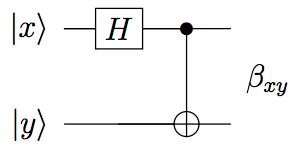
\includegraphics[width=4cm]{Figures/bell}
\end{center}

Es decir, partiendo del estado inicial \( \ket{xy} \), se aplica \textit{H} al primer qubit, y luego se aplica \textit{CNOT} a ambos, donde el primero es el de control (marcado con el punto negro). En otras palabras, este circuito representa la siguiente ecuación:
\[
  \beta_{xy} = CNOT(H \tensor I)\ket{xy}
\]
Las posibles salidas de este circuito, cuando \( x \) e \( y \) varían entre \( 0 \) y \( 1 \) son las siguientes:
\begin{equation*}
  \begin{split}
    \ket{00} \xrightarrow{H(1)} \frac{1}{\sqrt{2}} (\ket{0} + \ket{1})\ket{0} = \frac{1}{\sqrt{2}} (\ket{00} + \ket{10}) \xrightarrow{CNOT(1,2)} \frac{1}{\sqrt{2}} (\ket{00} + \ket{11}) = \beta_{00} \\
    \ket{01} \xrightarrow{H(1)} \frac{1}{\sqrt{2}} (\ket{0} + \ket{1})\ket{1} = \frac{1}{\sqrt{2}} (\ket{01} + \ket{11}) \xrightarrow{CNOT(1,2)} \frac{1}{\sqrt{2}} (\ket{01} + \ket{10}) = \beta_{01} \\
    \ket{10} \xrightarrow{H(1)} \frac{1}{\sqrt{2}} (\ket{0} - \ket{1})\ket{0} = \frac{1}{\sqrt{2}} (\ket{00} - \ket{10}) \xrightarrow{CNOT(1,2)} \frac{1}{\sqrt{2}} (\ket{00} - \ket{11}) = \beta_{10} \\
    \ket{11} \xrightarrow{H(1)} \frac{1}{\sqrt{2}} (\ket{0} - \ket{1})\ket{1} = \frac{1}{\sqrt{2}} (\ket{01} - \ket{11}) \xrightarrow{CNOT(1,2)} \frac{1}{\sqrt{2}} (\ket{01} - \ket{10}) = \beta_{11}
  \end{split}
\end{equation*}

A estos estados se los llama \textit{estados de Bell}. Estos son
estados entrelazados, es decir, estados que no pueden representarse como el producto tensorial de dos estados individuales.

Un par de qubits que se encuentren en un estado de Bell se conoce como \textit{par EPR}. El nombre se debe a que Einstein, Podolsky y Rosen propusieron en 1935 la existencia de un fenómeno por el cual, cuando se tiene un par entrelazado (representado físicamente, por ejemplo, por el spin de un par de electrones o la polarización de un par de fotones) y un estado del par colapsa como resultado de haber realizado una medición, el segundo también colapsará, independientemente de qué tan lejos se encuentren físicamente. Este comportamiento parecía físicamente imposible, por lo cual se lo denominó la \textit{paradoja EPR}. Durante mucho tiempo se pensó que esto se debía a que la formulación de la mecánica cuántica estaba incompleta y que debía ser extendida, pero eventualmente este fenómeno pudo ser verificado experimentalmente.

\subsection{Teleportación cuántica}\label{teleportation}

La teleportación cuántica es un proceso mediante el cual se pueden transmitir qubits de una ubicación a otra mediante la ayuda de la comunicación clásica y de la existencia de un estado de Bell compartido entre el origen y el destino.

Utilizando como ejemplo a los personajes clásicos Alice y Bob, los pasos a seguir son los siguientes:
\begin{enumerate}
  \item Alice y Bob preparan un estado de Bell.
  \item Alice se queda con el primer qubit del par y Bob se lleva el segundo.
  \item Alice aplica \textit{CNOT} entre el qubit a transmitir y su parte del estado de Bell, y luego Hadamard al primero.
  \item Alice realiza una medición sobre los dos qubits en su poder y envía el resultado de la medición (2 bits clásicos) a Bob.
  \item Bob aplica una transformación sobre su qubit, de acuerdo a los bits recibidos: \( Z^{b_1} X^{b_2} \).
\end{enumerate}

El circuito completo queda de la siguiente forma:

\begin{center}
  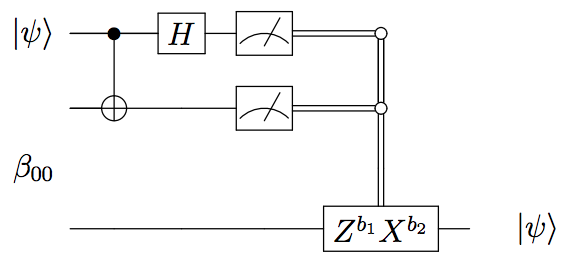
\includegraphics[width=6cm]{Figures/teleportation}
\end{center}

donde \( \ket{\psi} \) es el qubit a transmitir (o ``teleportar'').

Ejemplo: se quiere transmitir el qubit \( \ket{\psi} = \alpha \ket{0} + \beta \ket{1} \), entonces:
\begin{equation*}
  \begin{split}
    \ket{\psi} \tensor \beta_{00}
    & = (\alpha \ket{0} + \beta \ket{1}) \left(\frac{1}{\sqrt{2}} (\ket{0} + \ket{1}) \right) \\
    & = \frac{1}{\sqrt{2}} (\alpha \ket{0} (\ket{00} + \ket{11}) + \beta \ket{1} (\ket{00} + \ket{11})) \\
    & \xrightarrow{CNOT(1,2)} \frac{1}{\sqrt{2}} (\alpha \ket{0} (\ket{00} + \ket{11}) + \beta \ket{1} (\ket{10} + \ket{01})) \\
    & \xrightarrow{H(1)} \frac{1}{\sqrt{2}} \left( \alpha \frac{1}{\sqrt{2}} (\ket{0} + \ket{1})(\ket{00} + \ket{11}) + \beta \frac{1}{\sqrt{2}} (\ket{0} - \ket{1})(\ket{10} + \ket{01}) \right) \\
    & = \frac{1}{2} ( \ket{00} (\alpha \ket{0} + \beta \ket{1}) + \ket{01} (\alpha \ket{1} + \beta \ket{0}) \\
    & + \ket{10} (\alpha \ket{0} - \beta \ket{1}) + \ket{11} (\alpha \ket{1} - \beta \ket{0}) ) \\
    & = \frac{1}{2} \sum\limits_{b_1 = 0}^1 \sum\limits_{b_2 = 0}^1 \ket{b_1 b_2} (X^{b_2} Z^{b_1}) \ket{\psi}
  \end{split}
\end{equation*}

Por lo tanto, aplicando \( Z^{b_1} X^{b_2} \), Bob obtendrá el estado original \( \ket{\psi} \).

\section{\texorpdfstring{\( \lambdacalculus \)}{lambda calculus}}

El \( \lambdacalculus \) es un sistema formal introducido por Alonzo Church en 1930 para estudiar los fundamentos de la lógica y la matemática. Dicho cálculo posee dos simplificaciones que hacen que su semántica sea muy simple. La primera es que las funciones son tratadas como anónimas, es decir, no se les da un nombre. Por ejemplo, la función
\[ \mathsf{incrementar}(x) = x + 1 \]
puede ser reescrita anónimamente como
\[ (x) \mapsto x + 1 \]
Por otra parte, la función
\[ \mathsf{sumar}(x, y) = x + y \]
puede ser reescrita anónimamente como
\[ (x, y) \mapsto x + y \]
La segunda simplificación es que el \( \lambdacalculus \) solo considera funciones que tomen un solo argumento. Para representar funciones que tomen más de un argumento, como \textsf{sumar}, se puede representar como una función que tome un argumento, y como salida devuelva otra función que tome otro argumento. Por ejemplo,
\[ (x, y) \mapsto x + y \]
puede ser reescrita como
\[ x \mapsto (y \mapsto x + y) \]

A pesar de su simpleza, el \( \lambdacalculus \) puede ser utilizado para simular cualquier máquina de Turing. Esto significa que, dado cualquier modelo computacional, existe un equivalente en el \( \lambdacalculus \).
Por ejemplo, para modelar los números naturales y las operaciones sobre ellos, Church diseñó una codificación que lleva su nombre. En los siguientes ejemplos, vamos a asumir la existencia de los números naturales junto con el operador de suma (\( + \)), y al final de la sección mencionaremos cómo se modelan utilizando la codificación de Church.

La gramática de términos en forma BNF del \( \lambdacalculus \) es la siguiente\footnote{Para una introducción a gramáticas formales en \textit{Backus normal form}, ver, por ejemplo: \url{http://www.garshol.priv.no/download/text/bnf.html}}:
\[
  \tag{Términos}
  t \triangleq x \mid (\lambda x . t) \mid (\app{t}{t})
\]
Es decir, se tienen variables, que normalmente se notan utilizando \( x \), \( y \) o \( z \), funciones, que se notan \( \lcabstr{x}{t} \) y aplicaciones de un término \( t \) a otro término \( r \), notado simplemente \( \lcapp{t}{r} \).
Por ejemplo, \textsf{incrementar} se puede escribir en el \( \lambdacalculus \) como
\[ (\lambda x . x + 1) \]
Por otra parte, \textsf{sumar} puede ser escrita como
\[ (\lambda y (\lambda x . x + y)) \]

La gramática nos da la forma de construir términos válidos. Por otro lado, una regla de reescritura o reducción nos dice cómo se interpreta operacionalmente.
La regla de reducción del \( \lambdacalculus \) es la siguiente:
% \[
%   \tag{\(\alpha\text{-conversión}\)}
%   (\abstr{x}{t}[x]) \reducesto (\abstr{y}{t}[y])
% \]
\[
  \tag{\(\beta\text{-reducción}\)}
  ((\lambda x . t) r) \reducesto t [r/x]
\]
Es decir, el término \( \lcapp{\lcabstr{x}{t}}{r} \) puede ser reescrito en el término \( t \), donde todas las ocurrencias de \( r \) son reemplazadas por \( x \).
Por ejemplo, \( \mathsf{incrementar}(3) \) se puede computar como
\[ \lcapp{\lcabstr{x}{x + 1}}{3} \reducesto 3 + 1 \]
Por otra parte, \( \mathsf{sumar}(5, 6) \) se puede computar como
\[ \lcapp{\lcabstr{y}{\lcapp{\lcabstr{x}{x + y}}{5}}}{6} \reducesto \lcapp{\lcabstr{y}{5 + y}}{6} \reducesto 5 + 6 \]

Cabe destacar que en la primera reducción del ejemplo precedente, no se ha utilizado exactamente la regla. Efectivamente, la regla dice cómo reducir \( \lcapp{\lcabstr{x}{t}}{r} \), y en este ejemplo teníamos \( \lcapp{\lcabstr{y}{\lcapp{\lcabstr{x}{x + y}}{5}}}{6} \) para el cual la regla de reducción nos dice que debería reducir en \( \lcapp{\lcabstr{x}{x + 6}}{5} \). Lo que hicimos fue aplicar una regla de contexto. Las reglas de contexto del \( \lambdacalculus \) son las siguientes:
\[
  \quad\quad\quad
  \infer{\lcapp{t}{s} \reducesto \lcapp{r}{s}}{t \reducesto r}
  \quad\quad\quad\quad
  \infer{\lcapp{s}{t} \reducesto \lcapp{s}{r}}{t \reducesto r}
  \quad\quad\quad\quad
  \infer{\lcabstr{x}{t} \reducesto \lcabstr{x}{r}}{t \reducesto r}
\]
Con esta regla, sí podemos reducir \( \lcapp{\lcabstr{y}{\lcapp{\lcabstr{x}{x + y}}{5}}}{6} \) en \( \lcapp{\lcabstr{y}{5 + y}}{6} \), como hicimos en el último ejemplo.

En cuanto a los números naturales, estos pueden ser codificados de la siguiente forma:
\begin{equation*}
  \begin{split}
    0 & \triangleq \lcabstr{f}{\lcabstr{x}{x}} \\
    1 & \triangleq \lcabstr{f}{\lcabstr{x}{\lcapp{f}{x}}} \\
    2 & \triangleq \lcabstr{f}{\lcabstr{x}{\lcapp{f}{\lcapp{f}{x}}}} \\
    & \vdots
  \end{split}
\end{equation*}
Con respecto al operador de suma, este se modela esencialmente como la función que toma dos números codificados de esta forma, y produce la codificación correspondiente a la suma de ellos.

\section{\texorpdfstring{\( \lambdacalculus \)}{lambda calculus} simplemente tipado}

Consideremos el término \( \lcabstr{x}{\lcapp{x}{x}} \) del \( \lambdacalculus \) original, el cual aplicado a un término \( t \), posee el siguiente comportamiento:
\[
  \lcapp{\lcabstr{x}{\lcapp{x}{x}}}{t} \reducesto \lcapp{t}{t}
\]
Ahora consideremos qué ocurre si aplicamos \( (\lambda x . x x) \) a sí mismo:
\[
  \lcapp{\lcabstr{x}{\lcapp{x}{x}}}{\lcabstr{x}{\lcapp{x}{x}}} \reducesto \lcapp{\lcabstr{x}{\lcapp{x}{x}}}{\lcabstr{x}{\lcapp{x}{x}}}
\]
Vemos que al reducir el término \( \lcapp{\lcabstr{x}{\lcapp{x}{x}}}{\lcabstr{x}{\lcapp{x}{x}}} \) volvemos a obtener el mismo, sobre el cuál podemos volver a aplicar la misma regla de reducción. Es evidente que este término puede reescribir infinitamente.

Con el objetivo de excluir ciertos términos del \( \lambdacalculus \) original, en particular los términos que reescriben infinitamente, Alonzo Church introdujo en 1940 una extensión conocida como \textit{lambda cálculo simplemente tipado}. La idea consistía en introducir un sistema que permita asignar tipos a ciertos términos, excluyendo del lenguaje aquellos para los cuales un tipo no pueda ser asignado.

La sintaxis de términos del \( \lambdacalculus \) simplemente tipado es la siguiente:
\[
  \tag{Términos}
  t \triangleq x \mid \stlcabstr{x}{A}{t} \mid \stlcapp{t}{t}
\]
Por ejemplo, la función \textsf{incrementar} de la sección anterior se podría escribir como
\[ \stlcabstr{x}{\mathbb{N}}{x + 1} \]
o bien como
\[ \stlcabstr{x}{\mathbb{R}}{x + 1} \]
dependiendo del conjunto de números sobre la que la queramos definir.

Por otra parte, la sintaxis de tipos es la siguiente:
\[
  A \triangleq \tau \mid A \Rightarrow A \text{ donde } \tau \text{ es un tipo básico y } A \Rightarrow B \text{ el tipo función.}
\]

En cuanto a la semántica operacional, tenemos la siguiente regla de reducción (la cual coincide con la del \( \lambdacalculus \) original ignorando la notación de tipo):
\[
  \stlcapp{\stlcabstr{x}{A}{t}}{r} \reducesto t[r/x]
\]

Por ejemplo, \( \mathsf{incrementar}(3) \) se podría computar como
\[ \stlcapp{\stlcabstr{x}{\mathbb{N}}{x + 1}}{3} \reducesto 3 + 1 \]

Llamamos \textit{contexto} a un conjunto de variables tipadas y lo notamos con \( \Gamma \):
\[
  \Gamma \triangleq \vrbl{x_1}{A_1}, \ldots, \vrbl{x_n}{A_n}
\]

El \( \lambdacalculus \) simplemente tipado posee las siguientes reglas de tipado:

\begin{equation*}
  \infer{\Gamma \vdash x : A}{\vrbl{x}{A} \in \Gamma}
  \quad\quad\quad
  \infer{\Gamma \vdash \stlcabstr{x}{A}{t} : A \Rightarrow B}{\Gamma, \vrbl{x}{A} \vdash t : B}
  \quad\quad\quad
  \infer{\Gamma \vdash \stlcapp{t}{r} : B}{\Gamma \vdash t : A \Rightarrow B & \Gamma \vdash r : A}
\end{equation*}

Por ejemplo, suponiendo que ya sabemos que \( \Gamma \vdash 3 : \mathbb{N} \) y \( \Gamma, x : \mathbb{N} \vdash x + 1 : \mathbb{N} \), para derivar el tipo de la expresión \( \stlcapp{\stlcabstr{x}{\mathbb{N}}{x + 1}}{3} \) procedemos de la siguiente forma:
\[ \infer{\Gamma \vdash \stlcapp{\stlcabstr{x}{\mathbb{N}}{x + 1}}{3} : \mathbb{N}}{\infer{\Gamma \vdash \stlcabstr{x}{\mathbb{N}}{x + 1} : \mathbb{N} \Rightarrow \mathbb{N}}{\Gamma, \vrbl{x}{\mathbb{N}} \vdash x + 1 : \mathbb{N}} & \Gamma \vdash 3 : \mathbb{N}} \]

Por otra parte, no es posible derivar un tipo para la expresión \( \stlcapp{\stlcabstr{x}{\mathbb{N}}{x + 1}}{\pi} \) donde \( \pi : \mathbb{R} \). Esto significa que dicha expresión no es un término válido. Similarmente, es imposible asignarle un tipo a la expresión \( (\lambda x . x x)(\lambda x . x x) \), por lo cual esta expresión no corresponde a un término del \( \lambdacalculus \) simplemente tipado. Lo mismo ocurre con cualquier expresión que en el \( \lambdacalculus \) original resultaba en un término que reescribía infinitamente. Esta propiedad es la que se conoce como \textit{normalización fuerte}, y en el siguiente capítulo vamos a probar su existencia.
